\section{Velocity distributions}\label{sect:velocitydistributions}

%It is hard to imagine the discipline of astronomy progressing without the science and engineering of instrumentation making high precision observations a reality. We have described in the earlier sections how observations are essential to constrain our theories. In this section the observations performed as part of the work done in this thesis are covered in some detail.
%
%The data analysed in this thesis has been obtained using the Keck II telescope during three observation visits at the W.\ M.\ Keck Observatory located on the volcano Mauna Kea on the island of Hawai'i (aka The Big Island), in the state of Hawaii in the U.S.A. We recognise and acknowledge the very significant cultural role and reverence that the summit of Mauna Kea has always had within the indigenous Hawaiian community. We have been most fortunate to have had the opportunity to conduct observations from this mountain.
%
%The Keck II telescope has a primary mirror of $\sim 10$\,m in diameter and comprises 36 hexagon segments that work together as a single unit. A photograph of the primary mirror taken during the first observational visit is shown in Figure~\ref{fig:keckii}. The telescope is constructed such that different instruments can be mounted to analyse the light that the telescope is capturing. For our work we have used the NIRSPEC spectrometer \citep{mclean:98}.
%
%\begin{figure}[p]
%    \centering
%    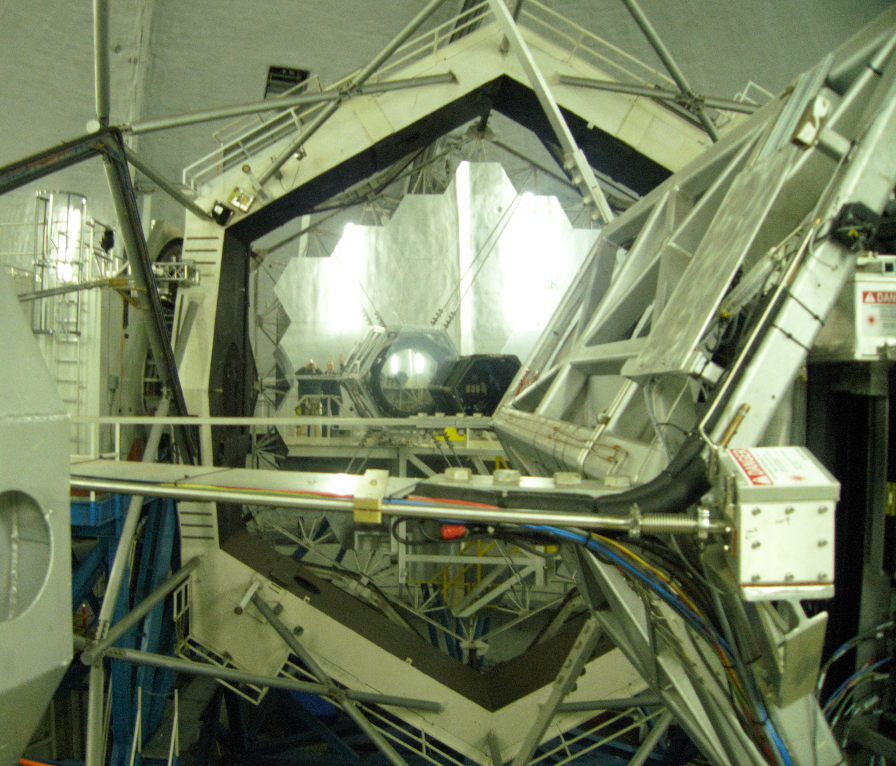
\includegraphics[width=1.0\textwidth]{images/keckii.png}
%    \caption{A photograph of the primary mirror of the Keck II telescope. The mirror is about 10\,m in diameter, illustrated by the size of the two people seen in the reflection (from the left Brian Thorsbro and Nils Ryde). The secondary mirror, which resides inside the metal box on the front right of the photograph, can be seen reflected in the primary mirror. The black hexagon, seen to the right of the reflection of the secondary mirror, is the focal point of the telescope where the captured light is gathered. From there the captured light is sent off to one of the mounted instruments. For our observations we used the NIRSPEC spectrometer that was mounted in one of the so-called Nasmyth/bent Cassegrain foci, located on the side of the telescope. Photograph by Brian Thorsbro.}
%    \label{fig:keckii}
%\end{figure}
%
%\begin{figure}[p]
%    \centering
%    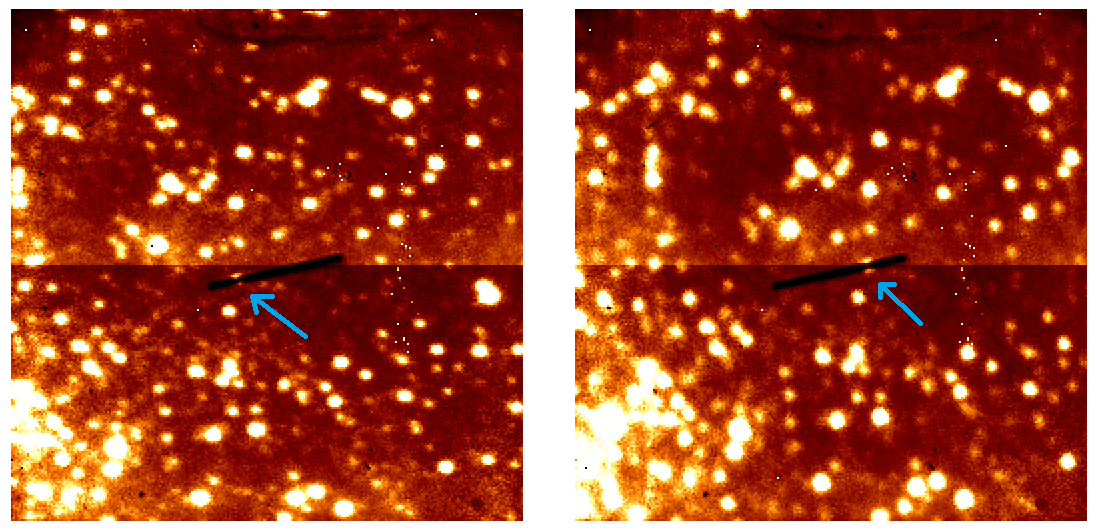
\includegraphics[width=1.0\textwidth]{images/gc13727scam.png}
%    \caption{Image taken with the Keck II telescope to verify that the target star, in this case the star named GC\,13727 in our work, is located correctly under the slit used to pass light on to the spectrometer. The blue arrows have been added to point out where the star is located. Two observations are performed using the ``nodding'' technique to ensure that it is also possible to obtain suitable background images for error subtraction.}
%    \label{fig:gc13727scam}
%\end{figure}
%\begin{figure}[p]
%    \centering
%    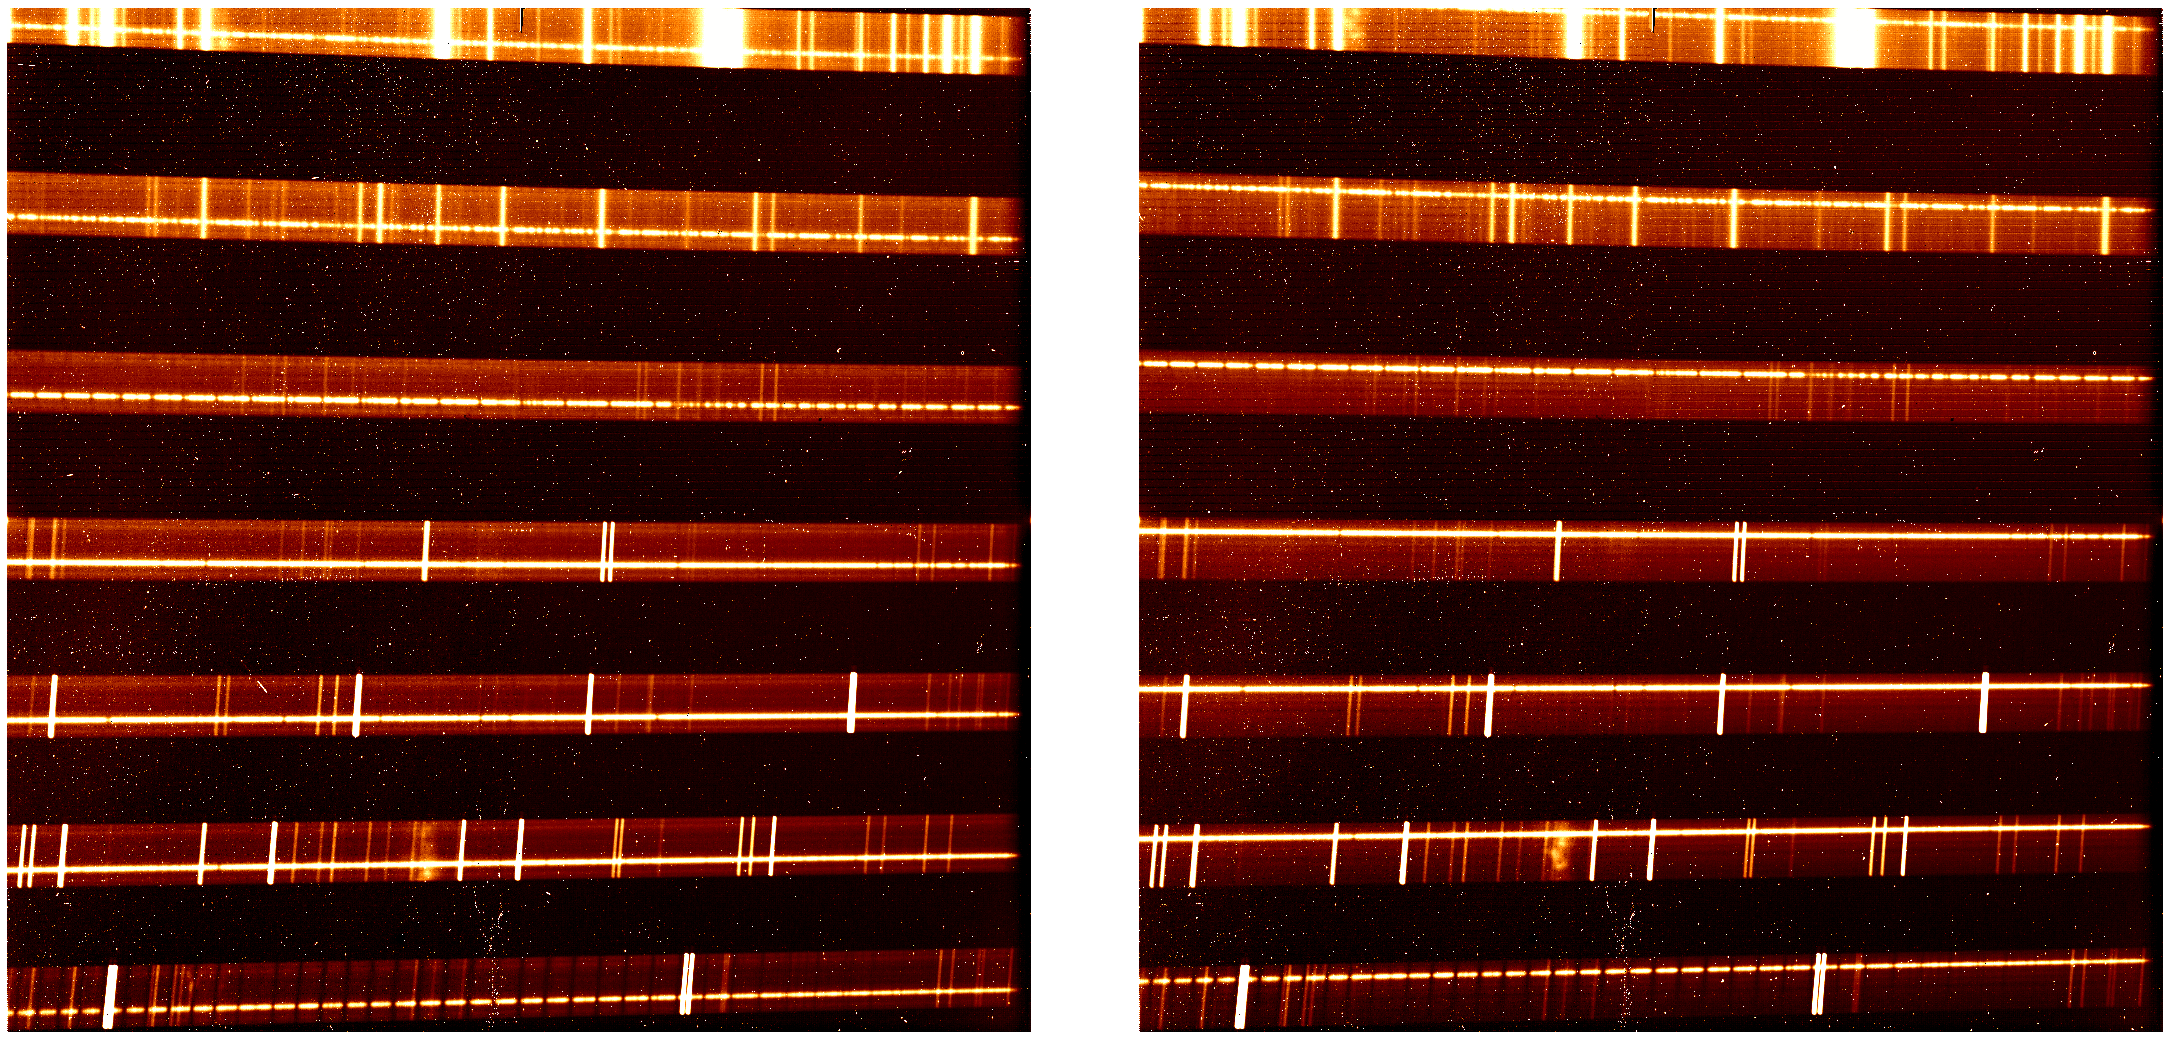
\includegraphics[width=1.0\textwidth]{images/gc13727speclight.png}
%    \caption{Observed cross-dispersed spectra of the same star, GC\,13727, as seen in Figure~\ref{fig:gc13727scam}. Absorption features can be seen as black ``Fraunhofer'' lines in various parts along the horizontal lines, which are the dispersed starlight. The vertical lines are OH emission lines from the Earth's atmosphere.}
%    \label{fig:gc13727spec}
%\end{figure}
%
%Observing the stars in the Galactic centre is particularly challenging because of the dust lying between the Sun and the Galactic centre. In the optical wavelength regime nearly all light is blocked. However, in the infrared wavelength regime around 2 micron about 15\% of the light penetrates through, which makes observations with large telescopes feasible. In our work we exposed the stars for about 40 minutes each on the Keck II telescope to reach a good signal to noise around 70 to 100. This is also the reason why we observe M giants, since they are very bright stars, with an apparent Ks magnitude around 11.
%
%The NIRSPEC spectrometer is a single slit spectrometer with a resolution of about R = 23,000. This is what we consider to be a necessary resolution for high quality abundance analyses. The slit of the spectrometer is placed on the star being observed, as illustrated in Figure~\ref{fig:gc13727scam}. We are interested in the light from the star, however the light passing through the rest of the slit can be used to quantify the background light. Subtracting background light allows for the reduction of systematic errors. This is especially important in the infrared, which is the wavelength region where we observe, since the thermal background is rather bright. Furthermore, there can be imperfections in the instrument that varies along the slit, so it is important to capture a background at the same slit location as the star, and to achieve this the telescope is ``nodded'', such that two observations are made. This way there will be two locations on the slit where the star is observed and for the same two slit positions there will also be a background observation. This ``nodding'' approach is shown in Figure~\ref{fig:gc13727scam} where blue arrows points to the location where the star is covered by the slit recording the light.
%
%The NIRSPEC spectrometer is a so-called cross-dispersed echelle spectrometer. This enables transverse dispersion of the recorded spectrum, such that a square detector array can be used more efficiently. In other words, the high resolution spectrum is cut up in parts and shifted vertically on the detector. An example of the image of a spectrum cut up in this way can be seen in Figure~\ref{fig:gc13727spec}. In this figure the horizontal lines are the spectrum of the observed star, and if one looks more closely it is possible to see black ``Fraunhofer'' lines, in particular in the third line from the top which displays molecular band absorption features of the molecule CO. The vertical lines are OH emission lines from Earth's atmosphere.
%
%In order to analyse the observed spectrum the spectral data has to be extracted from the image pixels. The Collaboration responsible for the design and implementation of the NIRSPEC spectrometer has made a software package available, called REDSPEC, which helps with this task \citep{nirspec_reduction}. The basic idea is to map out a curve that follows the spectrum across the pixels in the detector array and read out the intensity values along the curve. At the same time the software carries out background subtraction and divides out flat fields. The exact procedure will not be detailed here.
%
%Using the REDSPEC pipeline on the recorded image data we thus obtain a spectrum with an approximate wavelength calibration. Given that we observe in the infrared wavelength region around 2 microns we have many telluric features in the spectrum, which is both a blessing and a curse. It is helpful in improving the accuracy of the wavelength calibration, but it also means that parts of the spectrum are so crowded with telluric features that it can be difficult to reconstruct the actual stellar spectrum. Improving the wavelength calibration and removing the telluric features are performed by using the IRAF software package \citep{iraf}. For the telluric line removal we observe a swiftly rotating hot star which allows for easy identification of which spectral features that are telluric lines.
%
%However, in order to extract the abundances of chemical species, from the spectra that we observe we now turn to the field of stellar spectroscopy.
